% !TeX root = ..\main.tex
% Chapter 3

\chapter{系统设计与实现}

本章主要介绍本系统的设计与实现,包括系统的整体架构、各个模块的功能和实现方法。

\section{系统架构概述}
本系统包含图像分析、古诗生成、古诗评价和古诗优化四个模块,基于Python语言开发,使用百度智能云提供的API接口来调用模型,整体架构如图~\ref{fig:system_architecture}所示。

\begin{figure}[h]
    \centering
    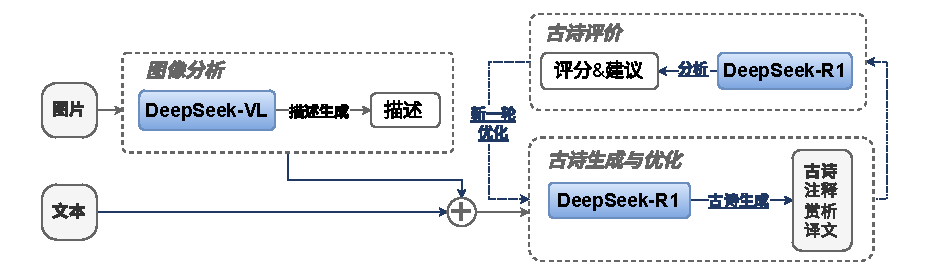
\includegraphics[width=1\textwidth]
    {figures/系统架构.pdf}\\
    \caption{系统架构}
    \label{fig:system_architecture}
  \end{figure}

\section{图像分析}

在先前的方案中,图像分析使用的是英文模型CLIP和MiniGPT-4,尽管生成的描述较精确、但无法捕捉有助于古诗创作的中国文化联想素材与情感色彩。因此,本系统使用DeepSeek-VL2\cite{wuDeepSeekVL2MixtureofExpertsVisionLanguage2024}替代之前的多模型组合方案,一步到位地为图像生成兼顾关键物体识别、整体场景信息和情感色彩的描述。(提示词见图~\ref{fig:prompt_image_analysis})

在调用百度智能云的API接口时,需要提供提示词和图像的URL地址,因此还需要将用户提供的图像上传到云端,并获得可公开访问的URL。为此,使用阿里云的对象存储OSS服务,利用OSS Python SDK,将用户图像上传到云端后,生成带有过期时间的GET方法预签名URL,供后续API调用使用。

\section{古诗生成}

在先前的方案中,古诗生成使用的是ERNIE-4.0模型,其无法在遵守韵律要求的同时充分运用经典典故意象,更别说提供使用典故的注释。因此,本系统使用DeepSeek-R1\cite{deepseek-aiDeepSeekR1IncentivizingReasoning2025},提示词设计参考CRISPE框架(提示词见图~\ref{fig:prompt_poem_generation})。

CRISPE框架包括六个部分:
\begin{enumerate}
  \item 能力与角色(Capacity and Role): 大模型应当具备的角色与能力。
  \item 背景信息(Insight): 为完成任务,大模型应当知晓的背景知识信息,以及用户需求的上下文语境。
  \item 指令(Statement): 大模型需要完成的任务。
  \item 输出风格(Personality): 大模型输出回复的风格、特色以及规范。
  \item 实验(Experiment): 尝试让大模型提供一些例子,以便更好地调试提示词。
\end{enumerate}

其中,最后投入使用的只包括前五个部分,而最后一个部分“实验(Experiment)”只是作调试用,方便提示词的设计迭代。

在生成古诗时,系统接收用户的文本输入\verb|user_text|,与用户输入图像的描述\verb|description|结合,同时指定古诗的体裁\verb|poem_type|(如五言绝句、七言律诗、不少于8句的排律等)。而除了古诗本身外,系统还会输出古诗的赏析、对古诗中典故的注释、以及白话文翻译,以便用户充分地理解古诗的意境、内涵和创作思路。


\section{古诗评价}

为了评价古诗的质量,本系统在自动度量方法的基础上,引入了DeepSeek-R1的评分机制。而为了使其能够给出合理、细致的评分,本文设计了一套包含五大维度的古诗评分体系(见表~\ref{tab:poem_scoring}),在先前工作的基础上,这套体系强调了对子维度中分数段的详细划分,并提供对应的示例以进一步阐明评分标准。基于这套评分体系,系统将逐一分析古诗的每个维度,给出分数和评语。此外,系统还将依照这套体系,逐一地给出修改意见,以提高古诗的质量。

由于评分体系较复杂、所占文本较多,提示词的设计参考了Few-shot框架\cite{brownLanguageModelsAre2020},在完成需求说明后,给定两个输入与输出的范例,确保模型按照预期的格式输出内容。(如图~\ref{fig:prompt_poem_analysis},其中两个输入输出示例如图~\ref{fig:example_poem_analysis_1}和图~\ref{fig:example_poem_analysis_2})于是,对先前生成的古诗(图~\ref{fig:example_poem}),系统的评分结果与优化建议如图~\ref{fig:example_analysis}和图~\ref{fig:example_suggestion}所示。

TODO 图例:雷达图

\begin{tcolorbox}[
  colback=white, % 背景透明
  colframe=black, 
  boxrule=1pt,        % 设置边框宽度
  arc=0mm             % 取消圆角
  ]
  \kaishu 
  [评分]\par
  1. 格律规范(21/25)\par
  \hspace{2em}1.1 平仄音韵(8/10):"琼英绽"三平尾(琼-平、英-平、绽-仄,按平水韵"绽"属谏韵为仄,实为三平调;"忍看落英飘"存在孤平现象\par
  \hspace{2em}1.2 对仗工稳(8/10):"琉璃映日"对"玉砌连云"器物建筑对仗精妙,但"曲径曾携"与"长亭忍看"动词结构稍欠工整\par
  \hspace{2em}1.3 押韵协调(5/5):全诗押平水韵二萧部(摇、桥、霄、飘、潮、遥、娇)如编钟贯珠\par
  2. 意象意境(27/30)\par
  \hspace{2em}2.1 古典运用(18/20):"晴川鹤影"化用崔颢典而不露,将"珞珈山"地域特征融入古典语境如盐入水\par
  \hspace{2em}2.2 意境层次(9/10):从实景(琼英绽)到追忆(书卷过)再到时空穿越(鹤影娇),构建三重意境如敦煌飞天飘带\par
  3. 主题思想(17/20)\par
  \hspace{2em}3.1 情感真挚(11/12):"青衿空对暮山遥"将求学记忆与离别惆怅交织,如吴带当风\par
  \hspace{2em}3.2 思想传承(6/8):"东君不解"暗合《楚辞》司春之神原型,但未突破传统伤春范式\par
  4. 语言锤炼(13/15)\par
  \hspace{2em}4.1 凝练度(7/8):"万点飞花迷画槛"数字量词精准如界画,唯"忍看"稍显直露\par
  \hspace{2em}4.2 典雅度(6/7):"粉泪"承李煜"胭脂泪"意象,"碧霄"接刘禹锡"晴空一鹤"语境\par
  5. 创新维度(8/10)\par
  \hspace{2em}5.1 守正出新(8/10):"珞珈山"地理符号与"金阙"仙家意象融合,如唐三彩吸收胡风\par
  总分:86/100
\end{tcolorbox}
\fakecaption{古诗评分(示例)}{fig:example_analysis}

\begin{tcolorbox}[
  colback=white, % 背景透明
  colframe=black, 
  boxrule=1pt,        % 设置边框宽度
  arc=0mm             % 取消圆角
  ]
  \kaishu 
  [改进建议]\par
  1. 格律规范\par
  \hspace{2em}1.1 平仄音韵:\par
  \hspace{2em}首联"琼英绽"改"琼瑶碎"(平平仄),既避三平调又暗含陆机《文赋》"玉卮无当,虽宝非用;琼瑶满案,终难为佩"的喻象\par
  \hspace{2em}"忍看落英飘"调整为"忍顾乱红凋"(仄仄仄平平),参考秦观"忍顾鹊桥归路"句式\par
  2. 意象意境\par
  \hspace{2em}2.1 古典运用:\par
  \hspace{2em}"晴川鹤影"可深化为"晴川历历汉阳树"的今昔对照,加入"残碑"意象与"鹤影"形成文明传承的张力\par
  \hspace{2em}"琉璃映日"建议改为"瑠璃承露",接续李贺"琉璃钟,琥珀浓"的瑰丽想象,增强晨昏时序感\par
  3. 主题思想\par
  \hspace{2em}3.2 思想传承:\par
  \hspace{2em}尾联注入《论语》"浴乎沂,风乎舞雩"的哲思,将"芳菲事"升华为"曾点之志",改"犹记晴川鹤影娇"为"独对春沂咏雩娇",使离愁转为文化坚守\par
  4. 语言锤炼\par
  \hspace{2em}4.1 凝练度:\par
  \hspace{2em}"朱阁檐前"精炼为"朱阑十二",化用李白"解释春风无限恨,沉香亭北倚阑干"的典故密度\par
  \hspace{2em}"香雪覆虹桥"调整为"香阵没星轺",借"星轺"(使者车驾)暗示人生旅途,增强叙事性\par
  5. 创新维度\par
  \hspace{2em}在"残红逐晚潮"处植入现代意象:"无人机影掠江皋",形成古典送别(兰舟)与当代离别(无人机)的蒙太奇,呼应李商隐"却话巴山夜雨时"的时空折叠技法\par

\end{tcolorbox}
\fakecaption{优化建议(示例)}{fig:example_suggestion}

此外,系统还将结合自动度量方法(BLEU、ROUGE、Similarity、Distinct)来进行指标计算,以辅助古诗的质量评估。

\section{古诗优化}

为了对生成的古诗进行优化,系统基于之前分析得到的改进意见,对古诗进行进一步的迭代润色,基于评分体系中的薄弱部分针对性地提高分数。

在先前的工作中,古诗优化的输入只包含待改进的古诗\verb|poem|和提供的修改意见\verb|suggestion|,这会导致两个问题——其一,修改意见\verb|suggestion|中的建议往往只包含那些明显不足的方面,并不能覆盖评分体系的所有维度,因此在优化时,模型很可能会忽略那些未被提及的维度,进而导致优化后的古诗在这些方面的分数下降,顾此而失彼;其二,在古诗优化时,模型只考虑了古诗的内容和结构,却没有考虑用户的原始输入,因此优化过程也可能会偏离用户的初衷,导致生成的古诗与用户的期望相去甚远。

因此,本系统在古诗优化时,除了原古诗\verb|poem|和改进建议\verb|suggestion|外,还增加了先前对原古诗的评分\verb|evaluation|和用户的输入(文本输入\verb|user_text|与图像输入描述\verb|description|),在确保古诗优化有效性的同时,保留对用户需求的考量。(如图~\ref{fig:prompt_poem_optimization})

于是,对先前生成的古诗(图~\ref{fig:example_poem}),结合图~\ref{fig:example_suggestion}中的优化建议,系统生成优化后的古诗(图~\ref{fig:example_poem_optimized}),并给出相应的优化说明(图~\ref{fig:example_poem_opt_explanation})。

\begin{figure}[ht]
  \centering
  \begin{tcolorbox}[
      colback=white,
      colframe=black,
      boxrule=1pt,
      arc=0mm,
      width=0.6\linewidth,  % 控制宽度
      ]
      \kaishu
      \centering
      珞珈山下琼瑶碎,朱阑十二翠云飘。\par
      万点飞花迷玉砌,千重香阵没星轺。\par
      瑠璃承露浮金阙,玉砌连云接碧霄。\par
      曲径曾携黄卷过,长亭忍顾乱红凋。\par
      东君未解青衿恨,犹遣残霞逐晚潮。\par
      粉泪暗随春水逝,素襟空对暮山遥。\par
      残碑鹤影参商渡,机影江声日夜迢。\par
      欲问蓬瀛何处是,春沂独咏舞雩娇。\par
  \end{tcolorbox}
  \caption{优化后古诗(示例)}
  \label{fig:example_poem_optimized}
\end{figure}

\begin{tcolorbox}[
  breakable,            % 允许跨页
  colback=white,
  colframe=black,
  boxrule=1pt,
  arc=0mm,
  % width=0.8\linewidth,  % 控制宽度
  ]
  \kaishu
  1. 平仄调整:"琼瑶碎"(平平仄)化解原三平尾,暗引陆机"琼瑶"喻指未琢之玉,喻学子未竟之志;"忍顾乱红凋"(仄仄仄平平)借易安"忍顾"词眼,使孤平转双拗救\par
  2. 意象重构:"朱阑十二"化用李白沉香亭典故,以数字阑干喻求学四载;"香阵没星轺"借骆宾王"香阵冲天"与谢灵运"星轺阻辙",喻青春壮志与宦途阻隔的冲突\par
  3. 时空折叠:新增颈联"残碑鹤影参商渡,机影江声日夜迢",以崔颢"晴川历历"对应珞珈残碑,无人机影接续李商隐"星桥铁锁"意象,构建古今送别对话场域\par
  4. 哲思升华:尾联化《论语》"风乎舞雩"为"春沂独咏",将樱花意象升华为"浴沂归咏"的文化坚守,使离愁转为对"曾点之志"的传承\par
  5. 器物对仗:调整"瑠璃承露"对"玉砌连云",既保持建筑意象,又以"承露"接续李贺琉璃钟意象,暗喻学子承接文化甘露\par
  6. 色彩体系:保留原诗"翠、金、碧、粉、青"色谱,新增"素襟"与"残霞"形成冷暖对照,暗合图片中琉璃瓦的冷绿与樱花的暖粉\par

\end{tcolorbox}
\fakecaption{优化说明(示例)}{fig:example_poem_opt_explanation}


\section{项目结构}

项目界面基于Gradio搭建。

TODO: <代码结构图>


TODO: <运行界面截图>